% Session 6 -- the Kitaev interaction: frustration that lives in the coupling, not in the lattice.
% Placement: sec. "Anisotropic exchange", in the Kitaev paragraph, after the H_Kitaev display.
% Rendered by figures/blender/s06f04_kitaev.py, labels in figures/overlays/s06f04_kitaev.tex.
\begin{aqmfigure}{fig:s06:kitaev}{The Kitaev interaction and the second kind of frustration. The
honeycomb lattice is bipartite, and its sites can be coloured with two colours, dark and light, as
in figure~\ref{fig:s06:frustration}(a). For this reason an ordinary Heisenberg antiferromagnet on
this lattice is not frustrated at all. The Kitaev coupling gives frustration anyway, because each of
the three bond directions, drawn in three styles, couples only \emph{one} spin component. The
$x$-bond only depends on $S^x$, so it favors both of its spins along $\pm\hat x$, the $y$-bond
favors $\pm\hat y$, and the $z$-bond favors $\pm\hat z$. Every site belongs to one bond of each
type, and no single orientation can satisfy three mutually orthogonal conditions at the same time,
which the three ghost arrows on the highlighted site show. Here the frustration comes from the
interaction and not from the geometry, and this is what makes the Kitaev model a paradigm for
quantum spin liquids in sessions 7 and 8.}
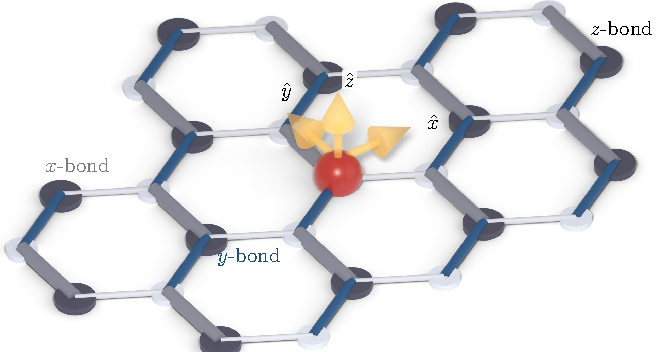
\includegraphics{figures/pdf/s06f04_kitaev.pdf}
\end{aqmfigure}
